% !TEX root = main.tex
\section{Limitierungen}
\label{sec:limitierungen}

Die wesentliche Limitierung von \textit{native image} ist die \textit{Closed-World}-Annahme. Das bedeutet, dass der gesamte Anwendungscode zur \textit{image build time} zur Verfügung
stehen muss. Java-Features die Nutzen von dynamischer Selbstbeobachtung (engl. dynamic introspection) machen (Reflection \& Dynamic Proxy) werden durch Konfigurationsdateien unterstützt.
Im Falle von Reflection werden in der Datei die individuellen Klassen, Methoden  und Felder angegeben die durch Reflection zugänglich sind. Bei Dynamic Proxy wird die Liste der Interfaces
angegeben die dynamische Proxies definieren. Durch die Nutzung von Konfigurationsdateien werden die dynamischen Inhalte bereits zur \textit{image build time}, also ahead-of-time, bekannt und
können aufgelöst werden. Um dem Entwickler Arbeit abzunehmen werden während des Buildvorganges automatisch statische Codeanalysen durchgeführt und die Konfigurationsdateien erstellt.

Features wie Dynamic Class Loading und InvokeDynamic, die zur Laufzeit dynamisch neuen Bytecode generieren oder Methodenaufrufe einfügen und ändern können, werden nicht unterstützt.
Auch der Security Manager wird nicht unterstützt, da es kein dynamisches Klassenloading gibt und dementsprechend nur vertrauenswürdiger Code ausgeführt wird \parencite{GraalLimitiations}.
Für eine vollständige Auflistung der Features und deren Unterstützung siehe Abbildung \ref{fig:system_limitations}.
\newpage
\begin{figure}[h]
	\centering
	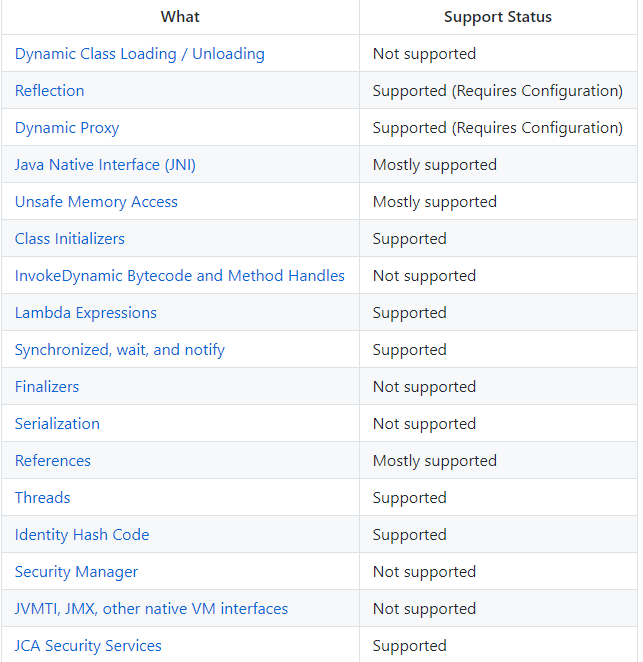
\includegraphics[width=1\textwidth]{resources/limitations.png}
	\caption{NativeImage Limitierungen \parencite{GraalLimitiations}}
	\label{fig:system_limitations}
\end{figure}
\newpage
